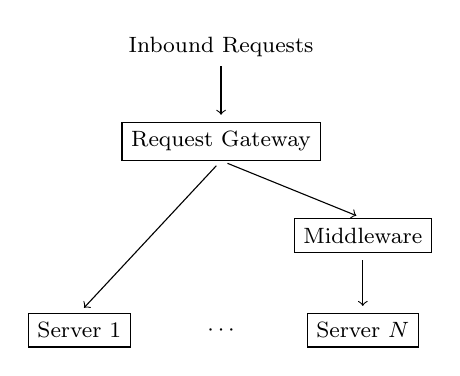
\begin{tikzpicture}[
	scale = 0.6,
	rect/.style={
		rectangle,
		draw=black
	},
	every node/.style={
		font=\footnotesize
	}
	]{
		\def\width{16}
		\def\height{9}
		%\draw[help lines, opacity=0.5] (0,0) grid (\width,\height);
		\node(p1) at (8,7) {Inbound Requests};
		\node[rect](g1) at (8,5){Request Gateway};
		\node[rect](s1) at (5,1){Server 1};
		\node(d1) at (8,1){\(\cdots\)};
		\node[rect](s2) at (11,1){Server \(N\)};
		\node[rect](s3) at (11,3){Middleware};
		
		\path[->, shorten >=0.25em] 										(p1.south) 	edge (g1.north);
		\path[->, shorten >=0.25em, shorten <=0.25em] 	(g1.south) 	edge (s1.north)
																																edge (s3.north);
		\path[->, shorten >=0.25em, shorten <=0.25em] 	(s3.south) 	edge (s2.north);																														
	}
\end{tikzpicture}